\chapternotnumbered{Introduction} \label{ch:Introduction}
\section{Instrumentation}
L'instrumentation regroupe \emph{les techniques, capteurs et systèmes} permettant 
de \emph{mesurer, surveiller et contrôler} des grandeurs physiques (température, pression, courant, etc.). Elle est omniprésente dans divers domaines scientifiques et technologiques : \emph{industrie, recherche, objets du quotidien, etc.}  

Ce domaine est essentiel dans de nombreuses applications :  
\begin{itemize}
  \item \textbf{Reconnaissance :} code-barres, badge RFID\footnote{Glossaire : \gls{rfid}}, etc.  
  \item \textbf{Industrie :} chaîne de montage, automatisation.  
  \item \textbf{Électroménager :} contrôle de température, détection d'ouverture.  
  \item \textbf{Santé :} mesure de la fréquence cardiaque, glycémie, pression artérielle.  
  \item \textbf{Automobile :} gestion du moteur, sécurité, freinage, direction.  
  \item \textbf{Domotique :} capteurs de mouvement, stores, fumée.  
\end{itemize}

\textbf{Instrumentation et applications spécifiques :}  
\begin{itemize}
  \item \textbf{Automobile :} une voiture moderne intègre des centaines de capteurs transmettant des données essentielles (\emph{température moteur, pression des pneus, trajectoire, niveaux d'huile et d'essence, etc.}).  
  \item \textbf{Domotique :} les capteurs contrôlent et automatisent les équipements (\emph{éclairage, chauffage, sécurité, volets, détecteurs de fumée, etc.}).  
  \item \textbf{Téléphonie :} les smartphones embarquent des capteurs pour \emph{mesurer la luminosité, la pression, l'orientation, le mouvement, la proximité, etc.}.  
\end{itemize}

\section{Internet of Things (IoT)}
L'IoT\footnote{Glossaire : \gls{iot}} prolonge l'instrumentation en intégrant \emph{connectivité et intelligence} aux capacités de mesure traditionnelles. Il repose sur un réseau d'objets connectés, équipés de capteurs et de logiciels, facilitant la collecte et l'échange de données.  

Ses caractéristiques principales incluent : \emph{connectivité, perception, analyse des données, interopérabilité, sécurité, évolutivité et expérience utilisateur.} Ces atouts permettent son adoption dans de nombreux secteurs, comme \emph{la santé, l'agriculture, les villes et maisons intelligentes, etc.}.

L'IOT doit suivre les caractéristiques suivantes:

\begin{itemize}
  \item \textbf{Connectivité :} les appareils IoT interagissent entre eux et avec 
  Internet pour \textit{échanger des données} et \textit{communiquer en temps réel}.  
  \item \textbf{Détection et analyse :} des capteurs collectent des informations de 
  l'environnement, puis les données sont traitées pour \textit{prendre des décisions} 
  et \textit{automatiser des processus}.  
  \item \textbf{Interopérabilité :} les dispositifs et systèmes hétérogènes 
  peuvent \textit{communiquer sans restrictions} pour fonctionner ensemble.  
  \item \textbf{Sécurité et confidentialité :} des mesures protègent les données 
  contre les accès non autorisés et garantissent leur intégrité.  
  \item \textbf{Évolutivité :} le réseau s'adapte à l'\textit{augmentation du 
  nombre d'appareils} sans dégradation des performances.  
  \item \textbf{Expérience utilisateur :} l'IoT vise une \textit{utilisation 
  intuitive} et une \textit{intégration fluide} dans le quotidien.
\end{itemize}


L'architecture IoT désigne l'organisation des composants interconnectés et leur interaction pour offrir une solution complète. Elle repose sur \textit{des appareils, capteurs, connectivité, applications et stockage}.  

L'architecture se structure en quatre couches :  
\begin{itemize}
  \item \textbf{Détection :} capteurs et actionneurs collectent des données sur l'environnement.  
  \item \textbf{Réseau :} assure la transmission des données via Bluetooth, Wi-Fi, réseaux cellulaires, etc.  
  \item \textbf{Traitement :} gère l'analyse des données, le stockage et la prise de décision.  
  \item \textbf{Application :} interface entre l'utilisateur et le système, incluant applications mobiles, Web et outils d'analyse.  
\end{itemize}

Un élément central de l'IoT est le \textbf{microcontrôleur (MCU)}, essentiel pour collecter et traiter les données des capteurs.


\section{Chaîne d'acquisition}

\begin{figure}[!ht]
  \centering
  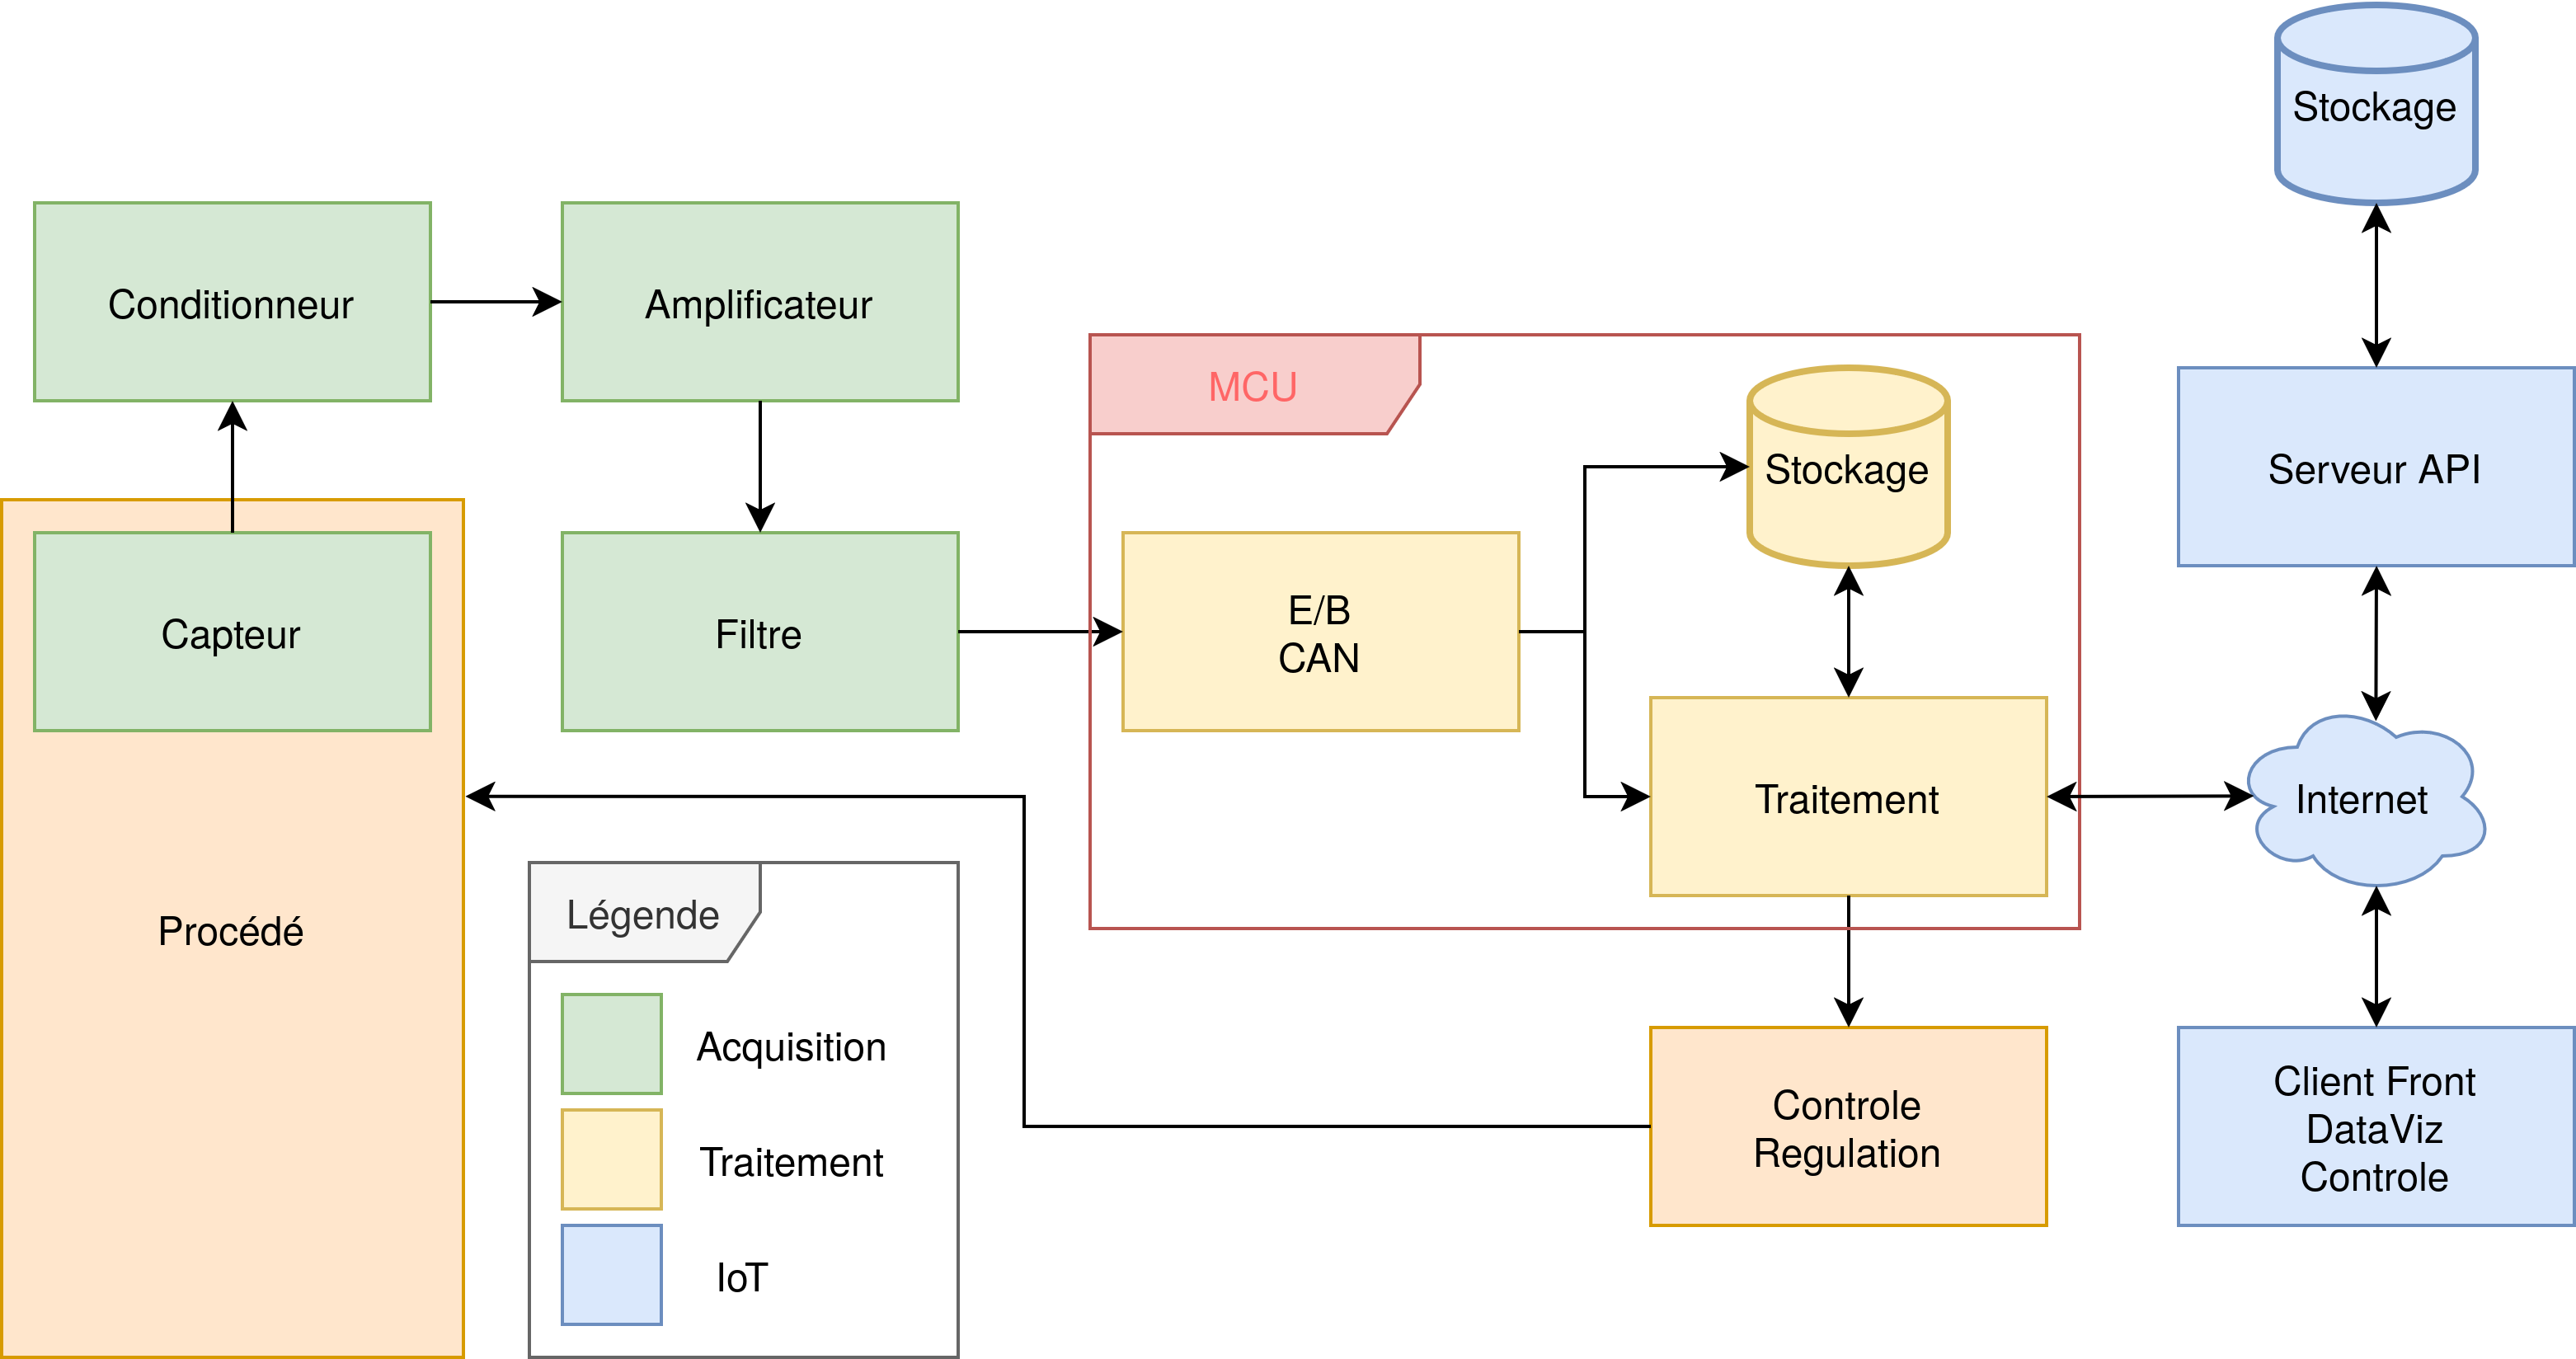
\includegraphics[width=0.9\textwidth]{chaine-acquisition}
  \caption{Chaîne d'acquisition}
  \label{fig:chain_acquisition}
\end{figure}